\documentclass[11pt]{article}

\usepackage[a4paper,margin=1in,top=1.1in,bottom=1.1in]{geometry}
\usepackage{amssymb}
\usepackage{xcolor}
\usepackage{tikz}
\usetikzlibrary{positioning,arrows.meta,shapes.geometric,fit,backgrounds,calc,matrix}
\usepackage{listings}
\usepackage{hyperref}
\usepackage{fancyhdr}
\usepackage{titlesec}
\usepackage{enumitem}
\usepackage{booktabs}
\usepackage{array}
\usepackage{microtype}
\usepackage{parskip}

% --- Palette (matches the dashboard) ---
\definecolor{bg}{HTML}{0E1116}
\definecolor{panel}{HTML}{161B22}
\definecolor{panel2}{HTML}{1F2630}
\definecolor{border}{HTML}{2A313C}
\definecolor{text}{HTML}{E6EDF3}
\definecolor{dim}{HTML}{8B949E}
\definecolor{pass}{HTML}{3FB950}
\definecolor{fail}{HTML}{F85149}
\definecolor{skip}{HTML}{484F58}
\definecolor{accent}{HTML}{1F6FEB}
\definecolor{accent2}{HTML}{6F42C1}
\definecolor{accentlight}{HTML}{DDF4FF}
\definecolor{accent2light}{HTML}{FBEFFF}
\definecolor{codebg}{HTML}{F4F5F7}
\definecolor{codeborder}{HTML}{D0D7DE}
\definecolor{codestr}{HTML}{0A3069}
\definecolor{codecmt}{HTML}{6E7781}
\definecolor{codekw}{HTML}{CF222E}

% --- Hyperlinks ---
\hypersetup{
  colorlinks=true,
  linkcolor=accent,
  urlcolor=accent,
  citecolor=accent,
  pdftitle={Meta-harness on Islo: a 200-line POC},
  pdfauthor={Yossi Eliaz (Incredibuild)},
  pdfsubject={Meta-harness optimization loop wired onto Islo sandboxes},
  pdfkeywords={meta-harness, islo, harbor, agent eval, harness optimization}
}

% --- Headings ---
\titleformat{\section}{\Large\bfseries\color{black}}{\thesection}{0.6em}{}
\titleformat{\subsection}{\large\bfseries\color{black}}{\thesubsection}{0.6em}{}
\setlength{\parskip}{0.5em}

% --- Code blocks ---
\lstdefinelanguage{shell}{
  morekeywords={islo,bin,bash,cd,ls,echo,cat,grep,fetch,python3,curl,git,gh,bin/meta-harness},
  morecomment=[l]\#,
  morestring=[b]",
  morestring=[b]',
}
\lstset{
  basicstyle=\ttfamily\small,
  backgroundcolor=\color{codebg},
  frame=single,
  framerule=0.4pt,
  rulecolor=\color{codeborder},
  framesep=6pt,
  xleftmargin=8pt,
  xrightmargin=8pt,
  keywordstyle=\color{codekw}\bfseries,
  stringstyle=\color{codestr},
  commentstyle=\color{codecmt}\itshape,
  showstringspaces=false,
  breaklines=true,
  breakatwhitespace=true,
  columns=fullflexible,
  keepspaces=true,
  literate=
    {—}{{\textemdash}}1
    {–}{{\textendash}}1
    {…}{{\ldots}}1
    {✓}{{\textcolor{pass}{\checkmark}}}1
    {✗}{{\textcolor{fail}{$\times$}}}1
    {│}{{\textbar}}1
    {└}{{\textbar}}1
    {├}{{\textbar}}1
    {─}{{-}}1
    {→}{{$\rightarrow$}}1,
}

% --- Headers/footers ---
\pagestyle{fancy}
\fancyhf{}
\renewcommand{\headrulewidth}{0pt}
\renewcommand{\footrulewidth}{0.4pt}
\fancyfoot[L]{\small\color{dim}meta-harness on Islo}
\fancyfoot[C]{\small\color{dim}\thepage}
\fancyfoot[R]{\small\color{dim}2026-05-05}

% --- Title block ---
\title{\vspace{-2em}\textbf{Meta-harness on Islo}\\[0.3em]
\large\normalfont A 200-line POC that goes from 0/5 to 5/5 in four proposer steps}
\author{\normalsize \textbf{Yossi Eliaz}\quad
  \textcolor{dim}{\small Incredibuild $\cdot$ Islo \quad
  \texttt{yossi.eliaz@incredibuild.com} $\cdot$ \texttt{yossi@islo.dev}}}
\date{\normalsize 2026-05-05}

\begin{document}

\maketitle
\thispagestyle{fancy}

\begin{center}
\textit{\color{dim}\small A small experiment in using Islo snapshots as the runtime for
\href{https://yoonholee.com/meta-harness/}{yoonholee's meta-harness} idea ---
and what the loop actually looks like when you wire it up end-to-end.}
\end{center}

\vspace{0.5em}
{\color{border}\hrule}
\vspace{1em}

% =================================================================
\section*{The idea, in one paragraph}

A \emph{harness} is the prompt + tools + scaffolding around an LLM agent. A
\emph{meta-harness} is the loop that improves the harness automatically: a
proposer agent reads the diagnostic logs of prior candidates, spots a failure
mode, and writes a better harness. Yoonho Lee's framing of the idea makes one
sharp claim: the bottleneck is \textbf{diagnostic context}. Most optimizers
compress prior runs into summary statistics; meta-harness gives the proposer
up to 10M tokens of raw execution traces to \texttt{grep} through.

That claim is only useful if the runtime can produce, store, and serve those
traces cheaply. Which is exactly what Islo sandboxes already do.

% =================================================================
\section*{The optimization loop, on Islo primitives}

\begin{center}
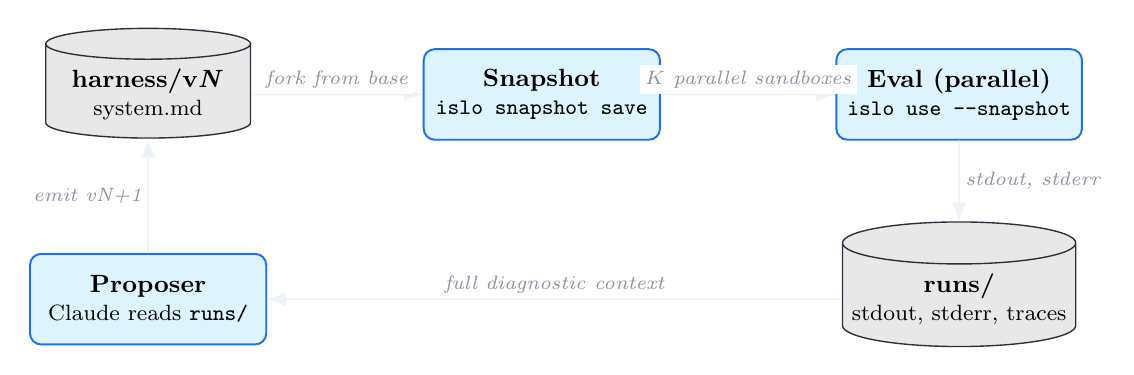
\begin{tikzpicture}[
  font=\small,
  every node/.style={align=center, font=\small},
  proc/.style={
    rectangle, rounded corners=4pt, draw=accent, line width=0.7pt,
    fill=accentlight, minimum width=3.0cm, minimum height=1.15cm, inner sep=4pt
  },
  store/.style={
    cylinder, shape border rotate=90, aspect=0.18, draw=border, line width=0.5pt,
    fill=panel!10, minimum width=2.6cm, minimum height=1.15cm
  },
  flow/.style={-{Latex[length=2.4mm]}, line width=0.6pt, draw=text!75},
  lbl/.style={font=\scriptsize\itshape, color=dim, fill=white, inner sep=2pt},
]
% Top row: harness ──► snapshot ──► eval
\node[store] (harness) at (0,0)   {\textbf{harness/v\textit{N}}\\[-1pt]\footnotesize system.md};
\node[proc]  (snap)    at (5,0)   {\textbf{Snapshot}\\[-1pt]\footnotesize\texttt{islo snapshot save}};
\node[proc]  (eval)    at (10.3,0){\textbf{Eval (parallel)}\\[-1pt]\footnotesize\texttt{islo use -{}-snapshot}};

% Bottom row: proposer ◄── runs
\node[proc]  (prop)    at (0,-2.6)  {\textbf{Proposer}\\[-1pt]\footnotesize Claude reads \texttt{runs/}};
\node[store] (runs)    at (10.3,-2.6){\textbf{runs/}\\[-1pt]\footnotesize stdout, stderr, traces};

% Top arrows
\draw[flow] (harness.east) -- node[lbl,above]{fork from base}             (snap.west);
\draw[flow] (snap.east)    -- node[lbl,above]{$K$ parallel sandboxes}     (eval.west);

% Right column: eval ──► runs (down)
\draw[flow] (eval.south)   -- node[lbl,right]{stdout, stderr}             (runs.north);

% Bottom arrow: runs ──► proposer (right to left)
\draw[flow] (runs.west)    -- node[lbl,above]{full diagnostic context}    (prop.east);

% Left column: proposer ──► harness (up)
\draw[flow] (prop.north)   -- node[lbl,left]{emit v\textit{N+1}}          (harness.south);
\end{tikzpicture}
\end{center}

\noindent Three things meta-harness needs from its runtime:

\begin{enumerate}[leftmargin=1.2em,itemsep=0.1em]
  \item \textbf{Reproducible eval environments} --- every candidate harness
        runs against the \emph{same} setup, otherwise the score is noise.
  \item \textbf{Massive parallelism} --- testing $N$ candidates $\times K$
        tasks adds up fast.
  \item \textbf{Persistent traces} --- the proposer needs to read
        stdout/stderr/agent-thoughts from runs that completed an hour ago.
\end{enumerate}

\noindent Islo's primitives map 1:1:

\begin{lstlisting}[language=shell]
islo snapshot save meta-base                  # prepare environment once
islo use mh-cand-7 --snapshot meta-base ...   # fork per candidate, in parallel
islo logs mh-cand-7 --type agent              # diagnostic traces, durable
\end{lstlisting}

Add \texttt{islo gateway} (deny-by-default egress, prevents reward-hacking)
and \texttt{-{}-source} \texttt{github://\allowbreak{}owner/\allowbreak{}repo}
(clones the workload at boot), and the wiring is basically free. Harbor ---
Islo Labs' \href{https://github.com/islo-labs/harbor}{framework for agent
evals and RL environments} --- slots in as the workload spec.

% =================================================================
\section*{The POC}

\begin{lstlisting}[language=shell]
tasks/        # 5 toy "SWE-style" tasks, each prompt.md + grade.sh
harness/v0/   # baseline system prompt, deliberately mediocre
bin/
  meta-harness    # bash orchestrator (eval | propose | loop | viz)
  agent-sim.py    # deterministic agent stand-in (offline mode)
  proposer.py     # reads runs/, emits harness/vN+1
viz/index.html    # live dashboard
runs/             # populated each iteration
\end{lstlisting}

\noindent Five tasks: FizzBuzz 1--15, first 10 primes, reverse a list, sum
even numbers in $[1..10]$, ``is racecar a palindrome.'' Each grades by
exact-match on stdout. Each has a known failure mode in v0 (off-by-one,
includes 1 as prime, comma vs space separator, exclusive vs inclusive bounds,
wrong case).

The agent is a Python simulator that's intentionally buggy --- until the
system prompt contains the right hint keyword. So the loop is
\emph{deterministic and offline}, runs in seconds, but the wiring is
identical to what you'd ship against real Claude on Islo.

The proposer is 80 lines: read \texttt{runs/iter-N/}, find which tasks
failed, look up the missing hint for that task, append it to a new
\texttt{harness/v\{N+1\}/system.md}. A real proposer would be:

\begin{lstlisting}[language=shell]
islo use --snapshot meta-base --agent claude --task "
  Examine /workspace/runs/iter-${N}. Find a common failure mode in the
  grade.sh stderr. Write /workspace/harness/v${N+1}/system.md as a small
  edit on top of v${N}/system.md to fix it."
\end{lstlisting}

Same input, same output contract. The orchestrator already has the stub.

% =================================================================
\section*{Results}

\subsection*{Pass-rate per iteration}

\begin{center}
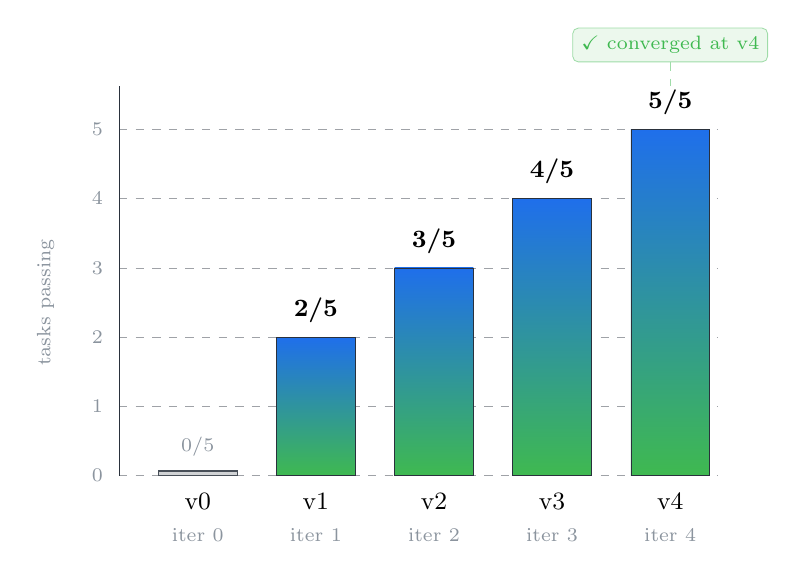
\begin{tikzpicture}[font=\small]
  \def\barW{1.0}
  \def\barGap{0.5}
  \def\maxH{4.4}
  \def\maxScore{5}
  \pgfmathsetmacro{\chartW}{4*(\barW+\barGap)+\barW}
  % Y axis + gridlines
  \draw[draw=border, line width=0.3pt] (0,0) -- (0,\maxH+0.55);
  \foreach \y in {0,1,2,3,4,5} {
    \pgfmathsetmacro{\yy}{\y/\maxScore*\maxH}
    \draw[draw=border, line width=0.2pt, dashed, opacity=0.45]
      (0,\yy) -- (\chartW+0.6,\yy);
    \node[anchor=east, font=\scriptsize\color{dim}] at (-0.08,\yy) {\y};
  }
  % Y-axis title
  \node[font=\scriptsize\color{dim}, rotate=90, anchor=south] at (-0.7, \maxH/2) {tasks passing};
  % Bars: (iter, harness, score, x-position-of-bar-left-edge)
  \foreach \i/\h/\s [count=\xi from 0] in {0/v0/0, 1/v1/2, 2/v2/3, 3/v3/4, 4/v4/5} {
    \pgfmathsetmacro{\xpos}{0.5+\xi*(\barW+\barGap)}
    \pgfmathsetmacro{\xc}{\xpos+\barW/2}
    \pgfmathsetmacro{\hh}{\s/\maxScore*\maxH}
    \ifnum\s=0
      \draw[draw=skip, line width=0.4pt, fill=skip!25]
        (\xpos,0) rectangle (\xpos+\barW, 0.06);
      \node[anchor=south, font=\scriptsize\color{dim}] at (\xc, 0.12) {\s/5};
    \else
      \shade[bottom color=pass, top color=accent]
        (\xpos,0) rectangle (\xpos+\barW, \hh);
      \draw[draw=border, line width=0.2pt]
        (\xpos,0) rectangle (\xpos+\barW, \hh);
      \node[anchor=south, font=\small\bfseries] at (\xc, \hh+0.06) {\s/5};
    \fi
    \node[anchor=north, font=\small] at (\xc, -0.1) {\h};
    \node[anchor=north, font=\scriptsize\color{dim}] at (\xc, -0.55) {iter \i};
  }
  % Convergence callout — sits clearly above the 5/5 label, with a thin
  % connector down to the v4 bar top so the association is unambiguous.
  \pgfmathsetmacro{\convX}{0.5+4*(\barW+\barGap)+\barW/2}
  \node[font=\scriptsize\color{pass}, anchor=south, fill=pass!10,
        rounded corners=2pt, inner sep=3pt, draw=pass!50, line width=0.3pt]
        (cv) at (\convX, \maxH+0.85) {$\checkmark$ converged at v4};
  \draw[draw=pass!50, line width=0.3pt, dashed]
        (\convX, \maxH+0.85) -- (\convX, \maxH+0.55);
\end{tikzpicture}
\end{center}

\subsection*{Task $\times$ iteration heatmap}

\begin{center}
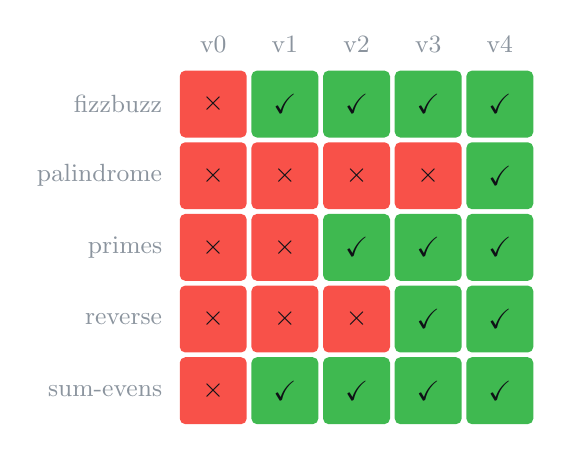
\begin{tikzpicture}[font=\small]
  \def\cell{0.85}
  \def\gap{0.06}
  % Tasks (rows) and iters (cols)
  \foreach \t/\name [count=\ti from 0] in {
      0/fizzbuzz, 1/palindrome, 2/primes, 3/reverse, 4/sum-evens
  } {
    \pgfmathsetmacro{\yy}{-\ti*(\cell+\gap)}
    \node[anchor=east, font=\small\color{dim}] at (-0.1, \yy-\cell/2) {\name};
  }
  \foreach \i/\h [count=\ii from 0] in {0/v0, 1/v1, 2/v2, 3/v3, 4/v4} {
    \pgfmathsetmacro{\xx}{\ii*(\cell+\gap)}
    \node[anchor=south, font=\small\color{dim}] at (\xx+\cell/2, 0.1) {\h};
  }
  % Status grid: row/col/state — 1=pass, 0=fail
  % rows: 0=fizzbuzz, 1=palindrome, 2=primes, 3=reverse, 4=sum-evens
  % cols: 0..4 = v0..v4
  \foreach \row/\col/\s in {
      0/0/0, 0/1/1, 0/2/1, 0/3/1, 0/4/1,
      1/0/0, 1/1/0, 1/2/0, 1/3/0, 1/4/1,
      2/0/0, 2/1/0, 2/2/1, 2/3/1, 2/4/1,
      3/0/0, 3/1/0, 3/2/0, 3/3/1, 3/4/1,
      4/0/0, 4/1/1, 4/2/1, 4/3/1, 4/4/1
  } {
    \pgfmathsetmacro{\xx}{\col*(\cell+\gap)}
    \pgfmathsetmacro{\yy}{-\row*(\cell+\gap)}
    \ifnum\s=1
      \fill[pass, rounded corners=2pt] (\xx,\yy) rectangle (\xx+\cell, \yy-\cell);
      \node[font=\bfseries, color=bg] at (\xx+\cell/2, \yy-\cell/2) {$\checkmark$};
    \else
      \fill[fail, rounded corners=2pt] (\xx,\yy) rectangle (\xx+\cell, \yy-\cell);
      \node[font=\bfseries, color=bg] at (\xx+\cell/2, \yy-\cell/2) {$\times$};
    \fi
  }
\end{tikzpicture}
\end{center}

\subsection*{What changed at each step}

\begin{center}
\renewcommand{\arraystretch}{1.25}
\begin{tabular}{@{}rlcl@{}}
\toprule
\textbf{iter} & \textbf{harness} & \textbf{score} & \textbf{what changed} \\
\midrule
0 & v0 & \textbf{0 / 5} & baseline --- minimal ``produce only the answer'' prompt \\
1 & v1 & \textbf{2 / 5} & + ``Loops are 1-indexed: count from 1 through N inclusive.'' \\
2 & v2 & \textbf{3 / 5} & + ``The smallest prime is 2 --- 1 is not prime.'' \\
3 & v3 & \textbf{4 / 5} & + ``Use space-separated output for separated values.'' \\
4 & v4 & \textbf{5 / 5} & + ``Format constraints are exact-case --- lowercase only.'' \\
\bottomrule
\end{tabular}
\end{center}

Five iterations. Four proposer steps. Hard cap was 10. Convergence was
diagnostic-driven: the proposer never saw the answer key, only
\texttt{grade.sh}'s exit code and one-line diff.

\subsection*{The interesting result: a free transfer-fix}

We added the hint targeting \textbf{fizzbuzz}, score went from 0/5 $\to$
2/5. The bonus point came from \texttt{sum-evens}: that task needed the
word \emph{``inclusive,''} and the fizzbuzz hint contained it (``count from
1 through N inclusive''). A free transfer-fix between two tasks with
overlapping vocabulary. A real proposer would either get more such accidents
(good) or learn to write more general hints on purpose (also good). This is
the kind of cross-trace insight you only see if the proposer can look at
\emph{all} the diagnostics, not summary stats.

% =================================================================
\section*{The visualization}

A single static HTML page (\texttt{viz/index.html}) polls
\texttt{runs/state.json} every 2 seconds and shows three things:

\begin{enumerate}[leftmargin=1.2em,itemsep=0.15em]
  \item \textbf{Pass-rate timeline} --- bars for each iteration, height = passing tasks.
  \item \textbf{Task $\times$ iteration heatmap} --- green/red grid, one cell per
        (task, harness). The shape of the green wave shows which tasks were
        fixed in which order, and whether any later iteration regressed an
        earlier pass.
  \item \textbf{Trace inspector} --- click any cell, see that run's stdout and
        the \texttt{grade.sh} stderr. This is the part that matters: it's the
        diagnostic surface the proposer is reading, made navigable for the
        human running the loop.
\end{enumerate}

You can also click a timeline bar to see the system prompt at that iteration,
with the newly-added section highlighted. Watching the prompt grow one rule
at a time is, weirdly, the most legible part of the whole thing --- it's the
harness \emph{learning to read its own task statements}.

\subsection*{Dashboard layout (sketch)}

\begin{center}
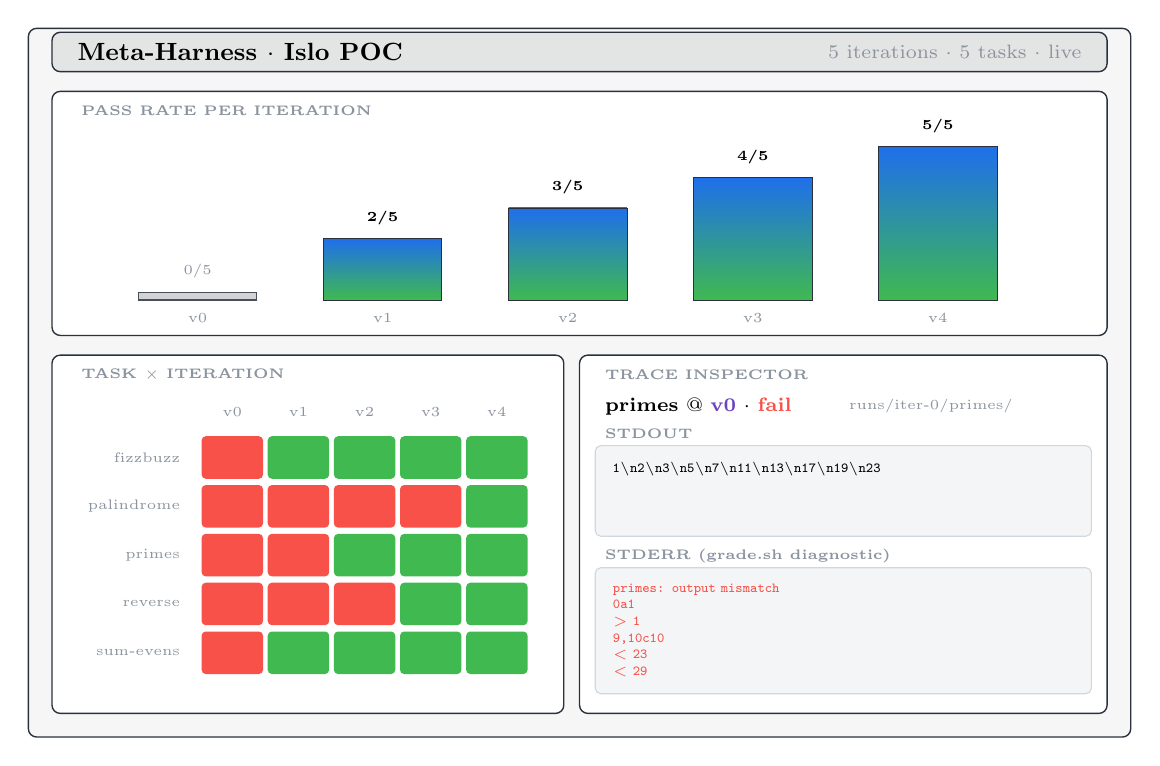
\begin{tikzpicture}[
  font=\scriptsize,
  panel/.style={rectangle, rounded corners=3pt, draw=border, fill=white, line width=0.5pt},
  hdr/.style={rectangle, rounded corners=3pt, draw=border, fill=panel!12, line width=0.5pt},
  sectlbl/.style={font=\tiny\bfseries, color=dim, anchor=west}
]
  % outer page
  \draw[panel, fill=panel!4] (0,0) rectangle (14,9);

  % header bar
  \draw[hdr] (0.30,8.45) rectangle (13.70,8.95);
  \node[anchor=west, font=\small\bfseries] at (0.50,8.70) {Meta-Harness $\cdot$ Islo POC};
  \node[anchor=east, color=dim] at (13.50,8.70) {5 iterations $\cdot$ 5 tasks $\cdot$ live};

  % ── Timeline panel ─────────────────────────────────────────────
  \draw[panel] (0.30,5.10) rectangle (13.70,8.20);
  \node[sectlbl] at (0.55,7.95) {PASS RATE PER ITERATION};
  \foreach \i/\score in {0/0, 1/2, 2/3, 3/4, 4/5} {
    \pgfmathsetmacro{\xL}{1.40+\i*2.35}
    \pgfmathsetmacro{\xC}{\xL+0.75}
    \pgfmathsetmacro{\h}{\score/5*1.95}
    \ifnum\score=0
      \draw[draw=skip, fill=skip!25] (\xL,5.55) rectangle (\xL+1.50,5.65);
      \node[anchor=south, font=\tiny, color=dim] at (\xC,5.70) {0/5};
    \else
      \shade[bottom color=pass, top color=accent]
        (\xL,5.55) rectangle (\xL+1.50,5.55+\h);
      \draw[draw=border, line width=0.2pt]
        (\xL,5.55) rectangle (\xL+1.50,5.55+\h);
      \node[anchor=south, font=\tiny\bfseries] at (\xC,5.55+\h+0.05) {\score/5};
    \fi
    \node[anchor=north, font=\tiny, color=dim] at (\xC,5.50) {v\i};
  }

  % ── Heatmap panel ──────────────────────────────────────────────
  \draw[panel] (0.30,0.30) rectangle (6.80,4.85);
  \node[sectlbl] at (0.55,4.60) {TASK $\times$ ITERATION};
  % row labels (anchored east, so right-edge sits at x=2.05; "fizzbuzz" extends back inside the panel)
  \foreach \name [count=\r from 0] in {fizzbuzz,palindrome,primes,reverse,sum-evens} {
    \pgfmathsetmacro{\yy}{3.55-\r*0.62}
    \node[anchor=east, font=\tiny, color=dim] at (2.05,\yy) {\name};
  }
  % column headers (above first row of cells)
  \foreach \i in {0,1,2,3,4} {
    \pgfmathsetmacro{\xC}{2.20+\i*0.84+0.39}
    \node[anchor=south, font=\tiny, color=dim] at (\xC,3.95) {v\i};
  }
  % cells
  \foreach \row/\col/\s in {
      0/0/0, 0/1/1, 0/2/1, 0/3/1, 0/4/1,
      1/0/0, 1/1/0, 1/2/0, 1/3/0, 1/4/1,
      2/0/0, 2/1/0, 2/2/1, 2/3/1, 2/4/1,
      3/0/0, 3/1/0, 3/2/0, 3/3/1, 3/4/1,
      4/0/0, 4/1/1, 4/2/1, 4/3/1, 4/4/1
  } {
    \pgfmathsetmacro{\xL}{2.20+\col*0.84}
    \pgfmathsetmacro{\yC}{3.55-\row*0.62}
    \ifnum\s=1
      \fill[pass, rounded corners=1.5pt] (\xL,\yC-0.27) rectangle (\xL+0.78,\yC+0.27);
    \else
      \fill[fail, rounded corners=1.5pt] (\xL,\yC-0.27) rectangle (\xL+0.78,\yC+0.27);
    \fi
  }

  % ── Trace inspector panel ──────────────────────────────────────
  \draw[panel] (7.00,0.30) rectangle (13.70,4.85);
  \node[sectlbl] at (7.20,4.60) {TRACE INSPECTOR};
  \node[anchor=west, font=\scriptsize] at (7.20,4.20)
    {\textbf{primes} @ \textcolor{accent2}{\textbf{v0}} $\cdot$ \textcolor{fail}{\textbf{fail}}};
  \node[anchor=west, font=\tiny, color=dim] at (10.30,4.20) {runs/iter-0/primes/};

  % stdout box
  \node[sectlbl] at (7.20,3.85) {STDOUT};
  \draw[draw=codeborder, fill=codebg, rounded corners=2pt]
    (7.20,2.55) rectangle (13.50,3.70);
  \node[anchor=north west, font=\ttfamily\tiny, color=black, text width=6.05cm] at (7.30,3.62)
    {1\textbackslash n2\textbackslash n3\textbackslash n5\textbackslash n7\textbackslash n11\textbackslash n13\textbackslash n17\textbackslash n19\textbackslash n23};

  % stderr box
  \node[sectlbl] at (7.20,2.30) {STDERR (grade.sh diagnostic)};
  \draw[draw=codeborder, fill=codebg, rounded corners=2pt]
    (7.20,0.55) rectangle (13.50,2.15);
  \node[anchor=north west, font=\ttfamily\tiny, color=fail, text width=6.05cm] at (7.30,2.07)
    {primes: output mismatch\\
     0a1\\
     \textgreater{} 1\\
     9,10c10\\
     \textless{} 23\\
     \textless{} 29};
\end{tikzpicture}
\end{center}

% =================================================================
\section*{What this points at}

This POC is intentionally tiny so the loop is observable in one screen.
Three obvious next steps:

\begin{itemize}[leftmargin=1.2em,itemsep=0.2em]
  \item \textbf{Real backend.} Swap \texttt{BACKEND=sim} for
        \texttt{BACKEND=islo}. Each candidate $\times$ task becomes one
        \texttt{islo use -{}-snapshot meta-base} call. With Islo's
        parallelism that's $\sim$5--10s per task, end-to-end iteration in
        under a minute.
  \item \textbf{Real workload.} Replace the toy tasks with
        \href{https://github.com/islo-labs/harbor}{Harbor} or
        \href{https://github.com/islo-labs/long-horizon}{long-horizon} tasks.
        The orchestrator doesn't care --- it only needs \texttt{prompt.md} +
        \texttt{grade.sh} shape.
  \item \textbf{Real proposer.} Replace \texttt{proposer.py}'s pattern-match
        with Claude reading the full \texttt{runs/} tree from inside a
        sandbox. This is where the 10M-token diagnostic context actually
        pays off --- and where you'd start seeing proposed \emph{tools}, not
        just prompt edits.
\end{itemize}

\textbf{Three swaps. Same orchestrator. Same dashboard. The wiring is the thing.}

\vspace{0.5em}
{\color{border}\hrule}
\vspace{0.6em}

\begin{center}
\small\color{dim}
Code: \texttt{bin/meta-harness demo} to run it; \texttt{bin/meta-harness viz} to watch it.\\
$\sim$600 lines including the dashboard, deliberately scrappy.\\[0.6em]
\href{https://github.com/zozo123/meta-harness-eng-islo}{\texttt{github.com/zozo123/meta-harness-eng-islo}}\\[0.2em]
Yossi Eliaz $\cdot$ Incredibuild $\cdot$ Islo\\[0.1em]
\texttt{yossi.eliaz@incredibuild.com} $\cdot$ \texttt{yossi@islo.dev}
\end{center}

\end{document}
